\usetikzlibrary{positioning}
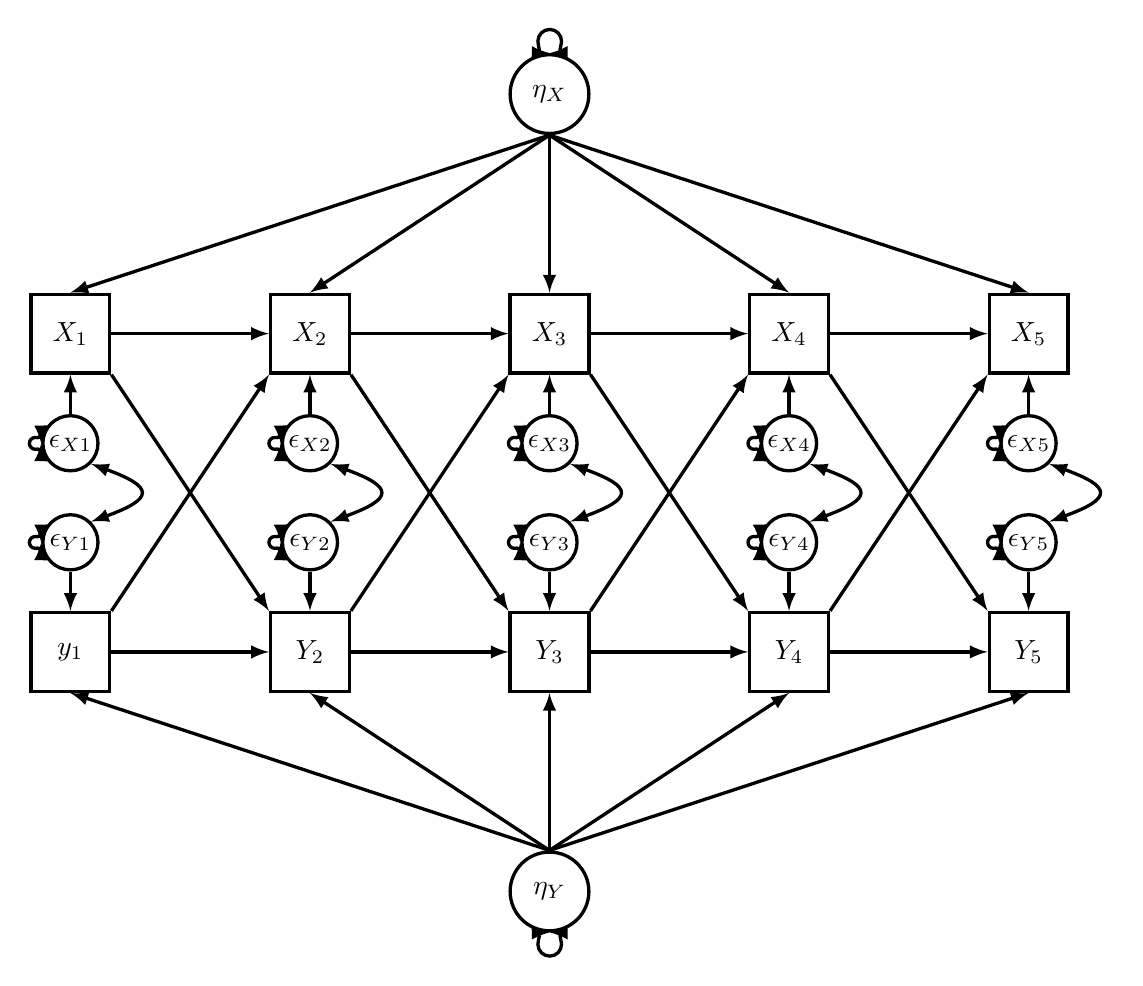
\begin{tikzpicture}[auto,node distance=.5cm, scale=0.5,
latent/.style={circle,draw,very thick,inner sep=0pt,minimum size=10mm,align=center},
manifest/.style={rectangle,draw,very thick,inner sep=0pt,minimum width=10mm,minimum height=10mm},
resid/.style={circle,draw,very thick,inner sep=0pt,minimum size=7mm,align=center},
paths/.style={->, very thick, -latex},
double/.style={very thick, latex-latex}
]
%create nodes
\node[manifest] (y1) at (0,0) {$y_1$};
\node[manifest, right=2cm of y1] (y2) {$Y_2$};
\node[manifest, right=2cm of y2] (y3){$Y_3$};
\node[manifest, right=2cm of y3] (y4){$Y_4$};
\node[manifest, right=2cm of y4] (y5){$Y_5$};

\node[manifest, above=3cm of y1] (x1){$X_1$};
\node[manifest, right=2cm of x1] (x2){$X_2$};
\node[manifest, right=2cm of x2] (x3){$X_3$};
\node[manifest, right=2cm of x3] (x4){$X_4$};
\node[manifest, right=2cm of x4] (x5){$X_5$};

\node[resid, below=0.5cm of x1] (ex1){$\epsilon_{X1}$};
\node[resid, below=0.5cm of x2] (ex2){$\epsilon_{X2}$};
\node[resid, below=0.5cm of x3] (ex3){$\epsilon_{X3}$};
\node[resid, below=0.5cm of x4] (ex4){$\epsilon_{X4}$};
\node[resid, below=0.5cm of x5] (ex5){$\epsilon_{X5}$};

\node[resid, above=0.5cm of y1] (ey1){$\epsilon_{Y1}$};
\node[resid, above=0.5cm of y2] (ey2){$\epsilon_{Y2}$};
\node[resid, above=0.5cm of y3] (ey3){$\epsilon_{Y3}$};
\node[resid, above=0.5cm of y4] (ey4){$\epsilon_{Y4}$};
\node[resid, above=0.5cm of y5] (ey5){$\epsilon_{Y5}$};

\node[latent, above=2cm of x3] (etax){$\eta_X$};
\node[latent, below=2cm of y3] (etay){$\eta_Y$};

%draw paths
\draw[paths] (ex1) -- (x1);
\draw[paths] (ex2) -- (x2);
\draw[paths] (ex3) -- (x3);
\draw[paths] (ex4) -- (x4);
\draw[paths] (ex5) -- (x5);

\draw[paths] (ey1) -- (y1);
\draw[paths] (ey2) -- (y2);
\draw[paths] (ey3) -- (y3);
\draw[paths] (ey4) -- (y4);
\draw[paths] (ey5) -- (y5);

\draw[paths] (x1.south east) -- (y2.north west);
\draw[paths] (x2.south east) -- (y3.north west);
\draw[paths] (x3.south east) -- (y4.north west);
\draw[paths] (x4.south east) -- (y5.north west);
\draw[paths] (y1.north east) -- (x2.south west);
\draw[paths] (y2.north east) -- (x3.south west);
\draw[paths] (y3.north east) -- (x4.south west);
\draw[paths] (y4.north east) -- (x5.south west);

\draw[paths] (x1.east) -- (x2.west);
\draw[paths] (x2.east) -- (x3.west);
\draw[paths] (x3.east) -- (x4.west);
\draw[paths] (x4.east) -- (x5.west);
\draw[paths] (y1.east) -- (y2.west);
\draw[paths] (y2.east) -- (y3.west);
\draw[paths] (y3.east) -- (y4.west);
\draw[paths] (y4.east) -- (y5.west);

\draw[paths] (etax.south) -- (x1.north);
\draw[paths] (etax.south) -- (x2.north);
\draw[paths] (etax.south) -- (x3.north);
\draw[paths] (etax.south) -- (x4.north);
\draw[paths] (etax.south) -- (x5.north);

\draw[paths] (etay.north) -- (y1.south);
\draw[paths] (etay.north) -- (y2.south);
\draw[paths] (etay.north) -- (y3.south);
\draw[paths] (etay.north) -- (y4.south);
\draw[paths] (etay.north) -- (y5.south);

%draw covariances of residuals
\draw[double] (ex1.south east) to [out=-20, in=20, looseness=3](ey1.north east);
\draw[double] (ex2.south east) to [out=-20, in=20, looseness=3](ey2.north east);
\draw[double] (ex3.south east) to [out=-20, in=20, looseness=3](ey3.north east);
\draw[double] (ex4.south east) to [out=-20, in=20, looseness=3](ey4.north east);
\draw[double] (ex5.south east) to [out=-20, in=20, looseness=3](ey5.north east);

%draw variance of latent factors
\draw[double] (etax.north) arc [start angle=269, end angle = -89, x radius = 0.3cm, y radius=0.3cm];
\draw[double] (etay.south) arc [start angle=-269, end angle = 89, x radius = 0.3cm, y radius=0.3cm];

%draw residual variances
\draw[double] (ex1.west) arc [start angle=1, end angle = 359, x radius = 0.15cm, y radius=0.15cm];
\draw[double] (ex2.west) arc [start angle=1, end angle = 359, x radius = 0.15cm, y radius=0.15cm];
\draw[double] (ex3.west) arc [start angle=1, end angle = 359, x radius = 0.15cm, y radius=0.15cm];
\draw[double] (ex4.west) arc [start angle=1, end angle = 359, x radius = 0.15cm, y radius=0.15cm];
\draw[double] (ex5.west) arc [start angle=1, end angle = 359, x radius = 0.15cm, y radius=0.15cm];

\draw[double] (ey1.west) arc [start angle=1, end angle = 359, x radius = 0.15cm, y radius=0.15cm];
\draw[double] (ey2.west) arc [start angle=1, end angle = 359, x radius = 0.15cm, y radius=0.15cm];
\draw[double] (ey3.west) arc [start angle=1, end angle = 359, x radius = 0.15cm, y radius=0.15cm];
\draw[double] (ey4.west) arc [start angle=1, end angle = 359, x radius = 0.15cm, y radius=0.15cm];
\draw[double] (ey5.west) arc [start angle=1, end angle = 359, x radius = 0.15cm, y radius=0.15cm];

\end{tikzpicture}